% ex: ts=2 sw=2 sts=2 et filetype=tex
% SPDX-License-Identifier: CC-BY-SA-4.0

\documentclass[10pt,addpoints]{exam}

\usepackage[utf8]{inputenc}
\usepackage[T1]{fontenc}
%\usepackage[spanish]{babel}
\usepackage[letterpaper]{geometry}
\usepackage{pgfplots}

\pagestyle{headandfoot}
\headrule
\header{Matemáticas aplicadas}{Examen Parcial III}{CBTIS 246}
\footer{}{Página \thepage\ de \numpages}{}

\pointpoints{punto}{puntos}
\renewcommand{\solutiontitle}{\textbf{Solución: }}

%\printanswers

\begin{document}
%\begin{center}
%\fbox{\fbox{\parbox{5.5in}{\centering
%Lee con atención cada pregunta y responde en
%el espacio ubicado en la parte izquierda.
%}}}
%\end{center}
%
%\vspace{5mm}

Nombre:\enspace\hrulefill

\vspace{5mm}

Grupo:\enspace\hrulefill
\enspace{}Grado:\enspace\hrulefill
\enspace{}Fecha:\enspace\hrulefill

\begin{questions}

% ex: ts=2 sw=2 sts=2 et filetype=tex
% SPDX-License-Identifier: CC-BY-SA-4.0

\question Usa la siguiente cuadricula para resolver los siguientes incisos:

  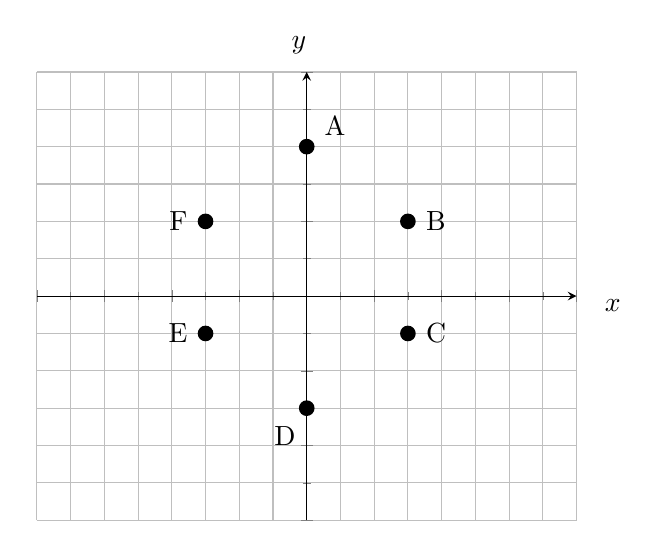
\begin{tikzpicture}
    \begin{axis}[grid=both,ymin=-6,ymax=6,xmax=8,xmin=-8,xticklabel=\empty,yticklabel=\empty,
               minor tick num=1,axis lines = middle,xlabel=$x$,ylabel=$y$,
               label style = {at={(ticklabel cs:1.1)}}]
      \node[label={10:{A}},circle,fill,inner sep=2pt] at (axis cs:0,4) {};
      \node[label={0:{B}},circle,fill,inner sep=2pt] at (axis cs:3,2) {};
      \node[label={0:{C}},circle,fill,inner sep=2pt] at (axis cs:3,-1) {};
      \node[label={260:{D}},circle,fill,inner sep=2pt] at (axis cs:0,-3) {};
      \node[label={180:{E}},circle,fill,inner sep=2pt] at (axis cs:-3,-1) {};
      \node[label={180:{F}},circle,fill,inner sep=2pt] at (axis cs:-3,2) {};
    \end{axis}
  \end{tikzpicture}

  \begin{parts}
    \part Encuantra las coordenadas de los vértices en el polígono. \\
    A(\fillin\ ,\fillin\ ) \enspace B(\fillin\ ,\fillin\ ) \\
    C(\fillin\ ,\fillin\ ) \enspace D(\fillin\ ,\fillin\ ) \\
    E(\fillin\ ,\fillin\ ) \enspace F(\fillin\ ,\fillin\ ) \\
    \part Determina el cuadrante en el que se ubica los puntos: \\
    El punto B esta en el cuadrante:\fillin \\
    El punto C esta en el cuadrante:\fillin \\
    El punto E esta en el cuadrante:\fillin \\
    El punto F esta en el cuadrante:\fillin \\
    \part Sacar la distancia entre los puntos: \\
    AB \fillin \enspace BC \fillin \enspace CD \fillin \\
    DE \fillin \enspace EF \fillin \enspace FA \fillin \\
    \part Calcula el perímetro de la figura resultante.
  \end{parts}


\newpage

% ex: ts=2 sw=2 sts=2 et filetype=tex
% SPDX-License-Identifier: CC-BY-SA-4.0

\question Se realiza una fuerza \fillin \enspace, cuando un cuerpo empuja
          a otro.

  \begin{oneparchoices}
    \choice De empuje
    \choice De velocidad
    \choice De fricción
    \CorrectChoice De contacto
  \end{oneparchoices}
  \answerline[D]

% ex: ts=2 sw=2 sts=2 et filetype=tex
% SPDX-License-Identifier: CC-BY-SA-4.0

\question Resuelve las siguientes ecuaciones y compruebalos sustituyendo el
          valor de $x$

  \begin{parts}
    \part $6x+4 = 3x+10$ \\
    \\
    \\
    \\
    \part $6x+3 = 2x+11$ \\
    \\
    \\
    \\
    \part $2x+5 = x-3$
  \end{parts}


\end{questions}

\end{document}
